\section{Description}
Consider the theater ticket reservation system.  You have built this system, 
and now you are responsible for the operation.  Your customer is quite happy 
with the system, except for the availability and, occasionally, the response 
time.  You’ve been in operation for 10 weeks.  To date, the availability of the
system components have been:
\begin{itemize}
    \item \textbf{Hardware} 99.9\%
    \item \textbf{Software}: 99.8\%
    \item \textbf{External Credit card verification and billing system}: 99.0\%
\end{itemize}
\noindent
The credit card system is required on only 30\% of all transactions, and the 
implementation allows other transactions and the system to work even if the 
credit card system is unavailable.

\pagebreak

\subsection{Calculate the system’s continuous availability percentage.}
The first step is to create a topology that explains how the system is integrated.
\begin{center}
    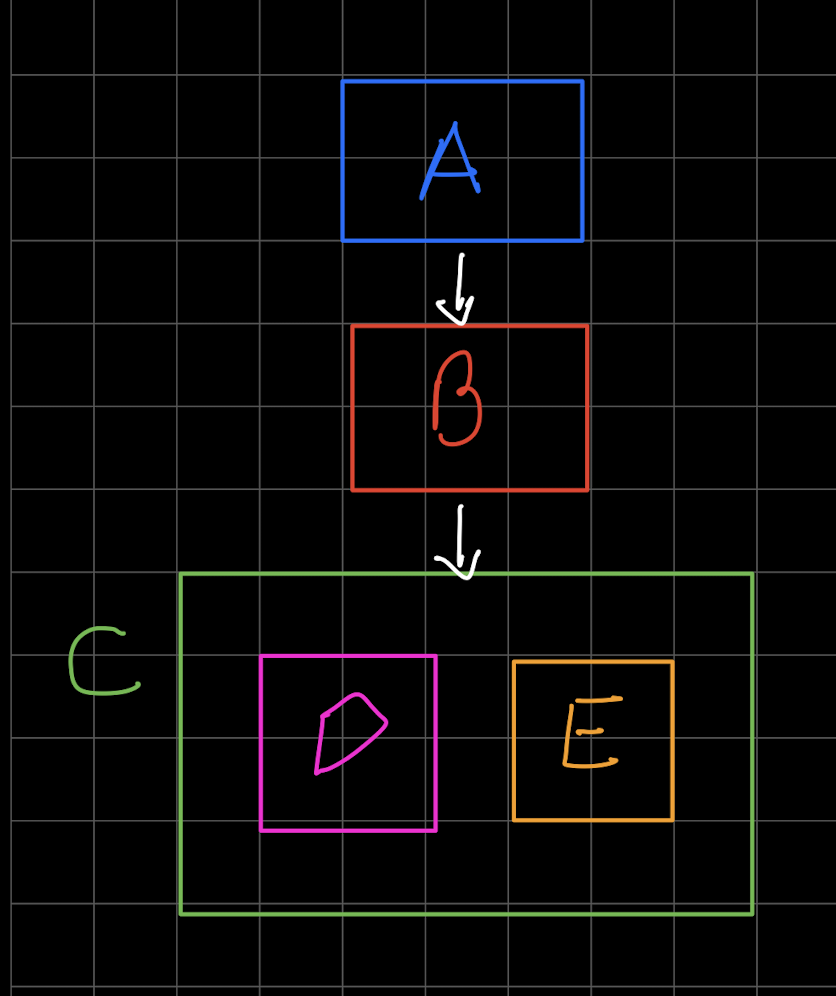
\includegraphics[scale=0.57]{diagram-1.png}    
\end{center}
\noindent
In this diagram, we have the Hardware as \textbf{A}, the software as \textbf{B} 
and we introduce a new abstraction that we will call \textit{Payment Module} as 
\textbf{C} know this payment module is going to handle all the transactions, it 
includes the \textbf{External Credit card verification and billing system} as a
submodule which we will call \textbf{D} and an internal billing module called 
\textbf{E}, which we are going to assume that is 100\% available. \newline\newline
\pagebreak

\noindent
\textit{Why did we did this?}\newline\newline

\noindent
Because the description says that 30\% of all transactions 
are credit card transactions which are handled by the component \textbf{D}, that 
means that the 70\% remaining transactions, let say cash, is handled 
by something else, that something else is the submodule \textbf{E}, both of 
this component work together to create the 
component \textbf{C}.\newline\newline
\noindent
Right now we know the availability of component \textbf{A} and \textbf{B}, but 
we need to calculate the availability of component \textbf{C}.
\[ C = D * 0.3 + E * 0.7 \]
\[ C = (0.99 * 0.3) + (1 * 0.7) \]
\[ C =  0.297 + 0.7 \]
\[ C =  0.997 = 99.7\% \]

\noindent
As we can see from the diagram, module \textbf{A}, \textbf{B} and 
\textbf{C} are in a serial configuration so the continuous availability 
\textbf{CA} would be \textbf{99.4\%}:
\[ CA = A(A) * A(B) * A(C) \]
\[ CA =  99.9\% * 99.8\% * 99.7\%\]
\[ CA =  0.999 * 0.998 * 0.997\]
\[CA = 0.994 = 99.4\%\]

\pagebreak

\subsection{Hot Backup System}
What would be the change in availability if you implement a hot backup system 
to reduce the scheduled maintenance time by 90\%? \newline

\noindent
We know that this change would be applied to the hardware, and we want to reduce 
the maintenance time, not the availability, by 90\%. First, we need to know 
what maintenance time is to see how much we are reducing, which 
is \textbf{1680} hours.
\[ Maintenance = 7 * 24 * 10 \]
\[ Maintenance = 1680 hours \]
Since we have a 99.9\% of availability right now, so we have \textbf{0.1\%} of
downtime due to maintenance. 
\[ Downtime = 1680 * 0.1 / 100 = 1.68 hours \]
If we reduce the downtime by 90\%, that means that the 10\% will tell us the 
final amount of downtime that we will have with the hot backup system which is 
\textbf{0.168} hours.
\[ Downtime = 1.68 * 10 / 100 = 0.168 hours \]
So the new availability for the hardware would be \textbf{99.99\%}: 
\[ A(A) = 100 - (100 * 0.168 / 1680) = 99.99\% \]

\pagebreak

\subsection{Improve the credit card vendor availability}
You know you need to improve the credit card vendor availability.  You search 
hard to find another credit card system vendor but can only find one whose 
availability is much worse (80\%).  still, you consider implementing it in 
addition to the first; that is, it is called if the first is unavailable.  
What would be the savings if you implemented this plan?

\begin{center}
    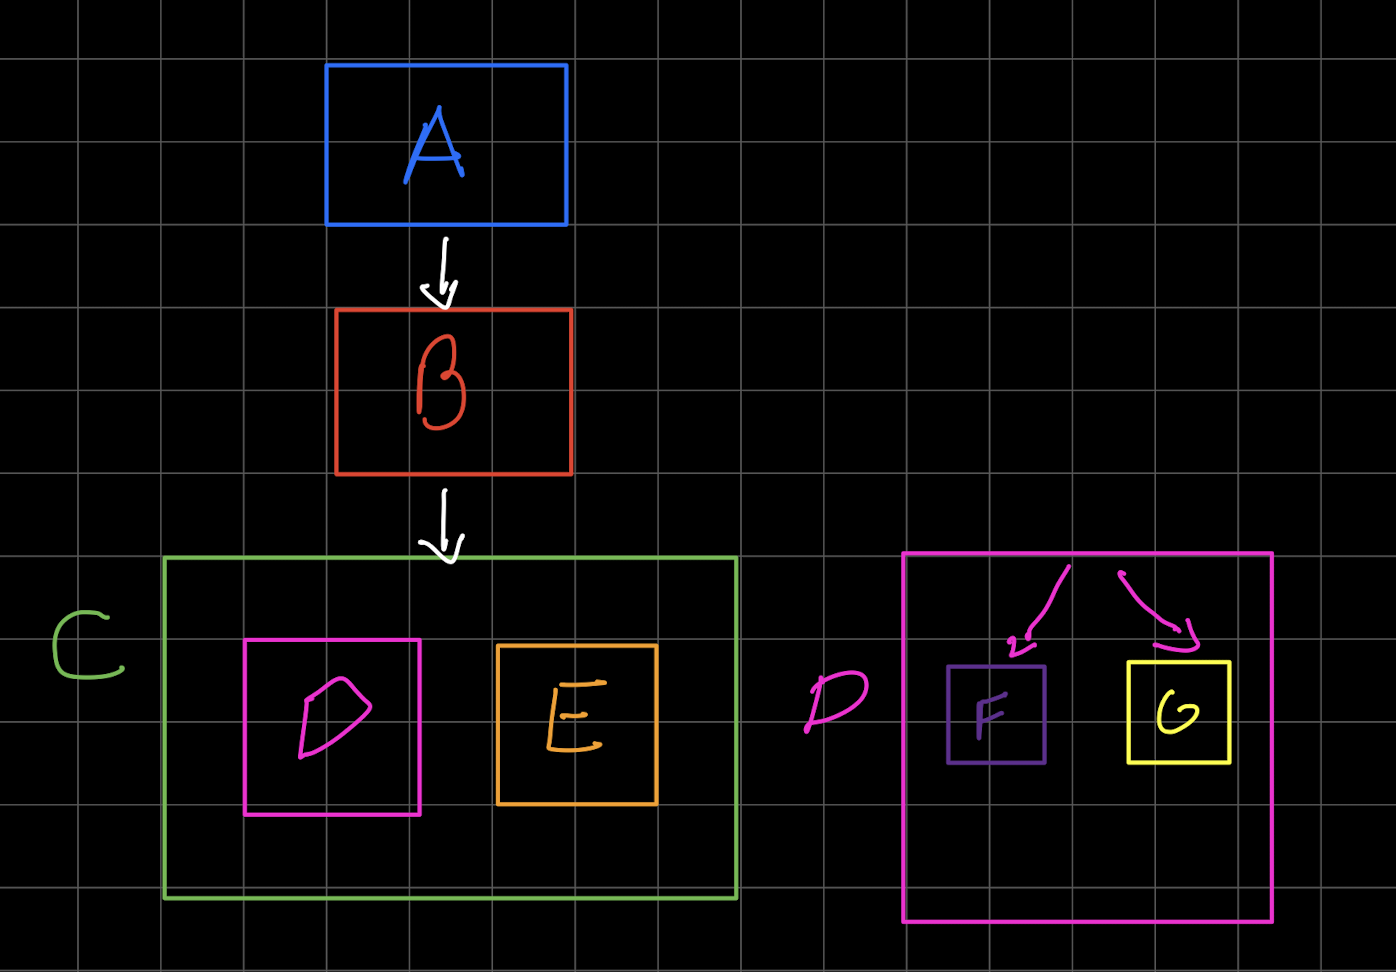
\includegraphics[scale=0.57]{diagram-2.png}    
\end{center}

\noindent 
Before we only have a single vendor which give the module \textbf{D} an 
availability of 99\%, now that we are introducing a new one we have two 
vendors in a parallel configuration that provides the service for the credit 
card.

\pagebreak
\noindent
The first thing we need to do is re-calculate the availability of 
module \textbf{D}, we have the submodule \textbf{F}, which is our original 
provider with 99\% of availability and we have the submodule \textbf{G}, our new 
vendor, with 80\% availability which give us a total of 
\textbf{99.8\%} availability.
\[ A(D) = 1 - (1 - 0.99) * (1 - 0.8) \]
\[ A(D) = 1 - (0.01) * (0.2) \]
\[ A(D) = 1 - 0.002 \]
\[ A(D) = 0.998 = 99.8\% \]
\noindent
This new vendor provides us with an increase of 0.8\% in availability, from 99\% 
to 99.8\%. This increase translates from 16.8 hours of downtime with 99\% availability
to 3.36 hours of downtime with 99.8\% which is 13.44 hour of uptime that we gain.
\[ Downtime(99\%) = 1680 * 0.01 = 16.8 hours\]
\[ Downtime(99.8\%) = 1680 * 0.002 = 3.36 hours\]
\[ Uptime Gained = 16.8 hours - 3.36 hours = 13.44 hours\]


\pagebreak

\subsection{Implementation of both plan}
If you implement both improvement plans, what is the projected 
availability of the system?\newline

\noindent
We need to calculate the new availability for module \textbf{C}, so we 
replace the availability of module \textbf{D} with its new availability.

\[ A(C) = D * 0.3 + E * 0.7 \]
\[ A(C) = (0.998 * 0.3) + (1 * 0.7) \]
\[ A(C) =  0.2994 + 0.7 \]
\[ A(C) =  0.9994 = 99.94\% \]

\noindent
With the implementation of the new vendor the availability of the 
module \textbf{C} becomes 99.94\%, now we re-calculate the availability of the 
whole system which is a serial configuration with the new availability for the 
module \textbf{A}, which gives us a total of \textbf{99.73\%} 
continuous availability.
\[ CA = A(A) * A(B) * A(C) \]
\[ CA =  99.99\% * 99.8\% * 99.94\%\]
\[ CA =  0.9999 * 0.998 * 0.9994\]
\[ CA = 0.9973 = 99.73\%\]

\pagebreak

\subsection{Degraded mode}
How might you use the concept of degraded mode to further improve the 
effective availability?\newline

\noindent
One way of using degraded mode will be if we do not process credit cards, and only
accept other types of transactions, that way 100\% of the transactions would be 
handled by the submodule \textbf{E} which in turn would increase the availability
of the module \textbf{C} to 100\%. So the effective availability, \textbf{EA}, 
for the system which only processes transactions with the 
submodule \textbf{E} would be \textbf{99.79\%}.

\[ EA = A(A) * A(B) * A(C) \]
\[ EA =  99.99\% * 99.8\% * 100\%\]
\[ EA =  0.9999 * 0.998 * 1\]
\[ EA = 0.9979 = 99.79\%\]

\pagebreak

\subsection{Response Time}
For the response time, the only problem seems to be that the credit card 
system responds either very quickly (< 1 second) or very slowly 
(15-20 seconds).  What should you do to improve your user satisfaction with 
the response time?\newline

\noindent
What we can do to improve user satisfaction could be handled by the interface 
itself, there is no need to involve a backend component, what we can do it's 
when we trigger the request in the client, by the client I mean client application 
(web interface, kiosk, computer application), we introduce an extra delay by 
the difference amount until we achieve 1 second, for example, if the request takes
500ms we introduced another 500ms to the loading spinner to make it look like 
it took longer, if the transaction takes longer than a second we do not introduce 
any extra time. \newline

\noindent 
The other involves transactions taking longer there are two approaches that we
can use from a UX perspective, one is, we block the UI and display a progress 
bar because progress bars make long tasks tolerable and the other option is 
to treat the transaction like a background task, meaning the application 
still handling the transaction but doesn't block the user from using the 
rest of the application.\newline

\noindent 
The loading blocking progress bar is easier to implement, the other background
task implementation requires keeping the state of the client, which one to use
depends on the context of the running application. \newline

\noindent
If the application only handles the purchase of a single ticket then the 
progress bar would be a better option because the user can't do anything 
else regardless. \newline

\noindent
If the ticket system enables to do other stuff like purchasing multiple 
tickets in parallel, choosing the seats in the event or updating the seats, 
then the background task the approach would be better because the user is 
not blocked to do other activities in the system.

